\section{Related Work}
\label{appendix:related_work}
\textbf{Generative LLM inference.} Taking OPT-175B as an example, assume 6 A100 80GB PCIe, based on the hardware specifications, we compare two main phases of inference time LLM, namely prompting and token generation in Table~\ref{table:obs_break_down_stage}, and two major components, namely Multi-Head-Attention block and MLP block in Table~\ref{table:obs_break_down_block}. In practice, the token generation phase usually dominates the end-to-end test latency due to IO latency. Generating only two tokens is about the same latency as prompting. Further, during token generation, the MLP block is 2 $\times$ more expensive in both FLOPs and IO access. The hardware is often at low utilization because memory reads and writes are more limited on modern hardware than tensor core computation.


 Given the rapid development of LLM, there is an emergence of systems that are specialized for LLM inference, such as Faster Transformer~\cite{nvidiaft},  Orca~\cite{yu2022orca}, LightSeq~\cite{wang2021lightseq}, PaLM inference~\cite{pope2022efficiently}, TurboTransformers~\cite{fang2021turbotransformers}, and Deepspeed-Inference~\cite{aminabadi2022deepspeed}. In practice, the token generation phase usually dominates the end-to-end inference time. Although the state-of-the-art systems introduce some helpful system optimizations for speedup, there is a lack of careful algorithm and system co-design to unleash the full potential of hardware efficiency during the LLM inference computation.   

\textbf{Near-neighbor Search for Efficient Deep Neural Networks.} Near-neighbor Search is a well-studied problem with wide applications in recommendation system~\cite{ xue2017deep,hall2015fast}, question answering~\cite{boytsov2016off,seo2019real, chang2020pre} and natural language processing~\cite{bengio2003neural,lee2015reasoning}. There has been a line of work using Near-neighbor Search techniques such as Locality-sensitive hashing~\cite{gionis1999similarity} and Graph-based indexing~\cite{malkov2014approximate} for efficient deep neural network training or inference~\cite{zhang2018navigating,chen2019fast,chen2020slide,kkl20,chen2021mongoose,chen2021scatterbrain,liu2022halos}.
% \subsection{Disecting LLM Test-Test Computation}



%  LLMs are commonly recognized as extremely computation hungry. However, there is a lack of understanding of the actual inference-time computation and IO, which is a must to pin out the latency bottleneck. In general, the generative procedure of LLM consists of two phases: i) the \textit{prompting} phase takes an input sequence to generate the \texttt{key} and \texttt{value} cache for each transformer block of LLM; and ii) the \textit{token generation} phase utilizes the \texttt{key} and \texttt{value} cache to generate tokens one after another.


% urther, due to the high dimensional of the MLP layer, for token generation, two MLP layers constitute0 the majority of FLOPs. In the case of OPT-175b, the MLP blocks consume 64.8\% of the FLOPS when processing texts of length 2048.
 % In general, the generative inference procedure of LLM consists of two phases: i) the \textit{prompt} phase takes an input sequence to generate the \texttt{key} and \texttt{value} cache (KV cache) for each transformer block of LLM; and ii) the \textit{token generation} phase utilizes and updates the KV cache to generate tokens step by step, where the current token generation sequentially depends on previously generated tokens. In practice, the token generation phase usually dominates the end-to-end inference time. Although the state-of-the-art systems introduce some helpful system optimizations for speedup, there is a lack of careful algorithm and system co-design to unleash the full potential of hardware efficiency during the LLM inference computation.   
% \begin{wrapfigure}{r}{0.2\textwidth}
%   \begin{center}
%     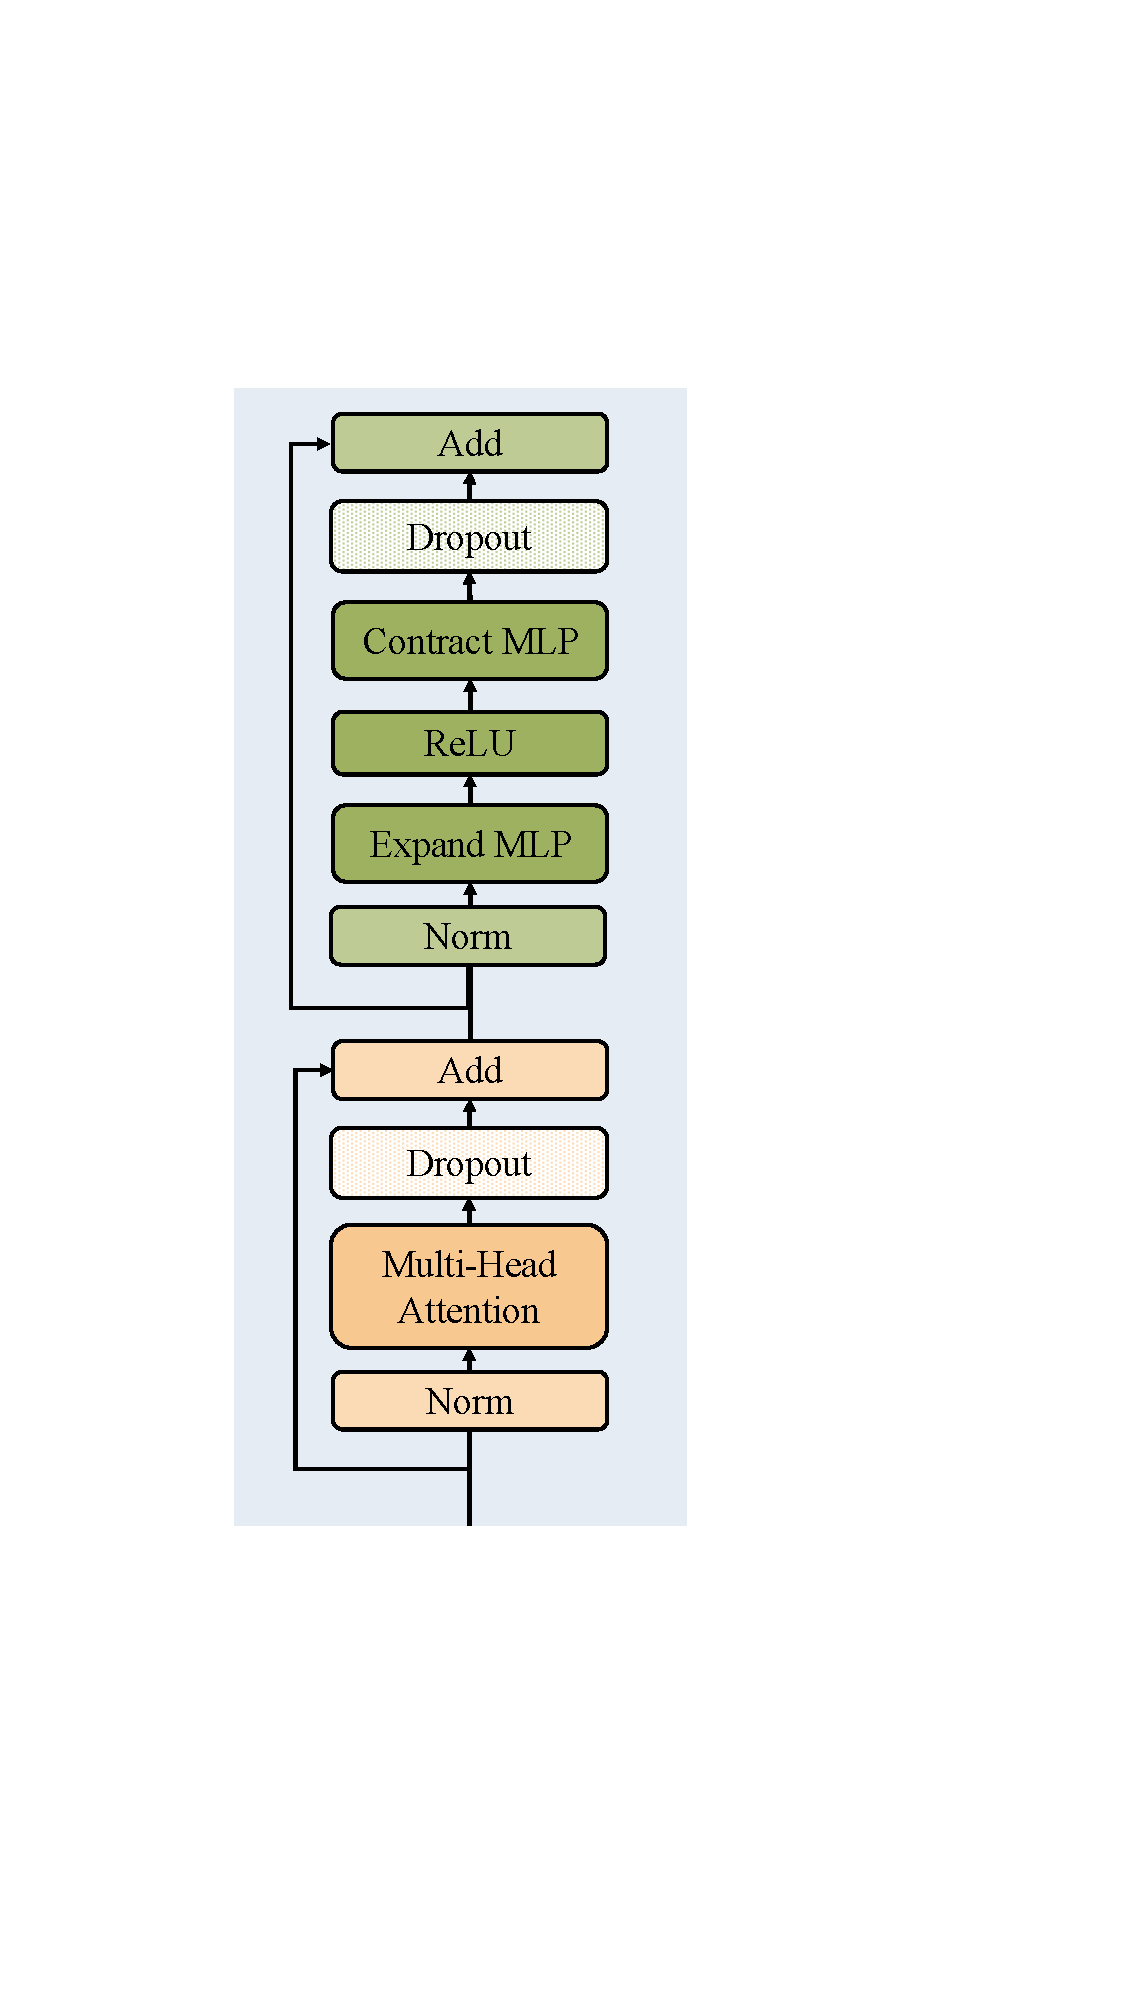
\includegraphics[width=0.18\textwidth]{figure/GPT_Blog_Diagram.pdf}
%   \end{center}
%   \vspace{-4mm}
%     \label{fig:arch}
%     \caption{OPT Architecture}
%       \vspace{-2mm}
% \end{wrapfigure}

\noindent \textbf{Quantization, pruning, distillation for LLM inference.} Various system relaxations have been studied for decades for model inference in machine learning. For example, quantization~\cite{han2015deep, jacob2018quantization,nagel2019data,zhao2019improving}, pruning~\cite{molchanov2016pruning,liu2018rethinking,he2019filter,hoefler2021sparsity}, and distillation~\cite{hinton2015distilling,cho2019efficacy,tang2019distilling,touvron2021training}  have been applied to speed up the inference of the machine learning model. Active research has recently attempted to apply such techniques in LLM inference. For example, zeroQuant~\cite{yao2022zeroquant} and nuQmm~\cite{park2022nuqmm} implement customized CUDA kernels to support tenor-wise or group-wise quantization for LLM inference; LLM.int8 \cite{dettmers2022llm} adopts a mixed \texttt{INT8/FP16} computation to diminish the influence of activation outliers; SmoothQuant~\cite{xiao2022smoothquant} enables efficient 8-bit weight and activation for LLM inference; GPTQ~\cite{frantar2022gptq} adopts a one-shot weight quantization method based on approximate second-order information for accuracy and efficiency; SparseGPT~\cite{frantar2023massive} introduces an approximate sparse regression solver to enable the sparsity in LLM inference; \cite{bansal2022rethinking} has reported that a small set of attention heads can perform primitive induction operations associated with in-context learning, and use this property to prune LLM for acceleration. 

%subsection{Various versions of the efficient large language model.}



%\subsection{Quantization, pruning, distillation}
%old techniques from 1990. no matter image or language


\noindent \textbf{Residual connections in neural networks.} Residual connection shows great advantages for neural network generalization, it provides additional paths for activations to reach the latter parts of the neural network by skipping some layers~\cite{he2016deep}. The advancement of residual connections can be viewed as ensembles of multiple shallow neural networks~\cite{veit2016residual}. Plenty of active research has discussed the effectiveness of residual connections~\cite{balduzzi2017shattered,bello2021revisiting,allen2019can,frei2019algorithm}. However, as far as we know, there is no former work that leverages the property of residual connections to improve the efficiency of LLM inference.  


